\documentclass[11pt,preprint, authoryear]{elsarticle}

\usepackage{lmodern}
%%%% My spacing
\usepackage{setspace}
\setstretch{1.2}
\DeclareMathSizes{12}{14}{10}{10}

% Wrap around which gives all figures included the [H] command, or places it "here". This can be tedious to code in Rmarkdown.
\usepackage{float}
\let\origfigure\figure
\let\endorigfigure\endfigure
\renewenvironment{figure}[1][2] {
    \expandafter\origfigure\expandafter[H]
} {
    \endorigfigure
}

\let\origtable\table
\let\endorigtable\endtable
\renewenvironment{table}[1][2] {
    \expandafter\origtable\expandafter[H]
} {
    \endorigtable
}


\usepackage{ifxetex,ifluatex}
\usepackage{fixltx2e} % provides \textsubscript
\ifnum 0\ifxetex 1\fi\ifluatex 1\fi=0 % if pdftex
  \usepackage[T1]{fontenc}
  \usepackage[utf8]{inputenc}
\else % if luatex or xelatex
  \ifxetex
    \usepackage{mathspec}
    \usepackage{xltxtra,xunicode}
  \else
    \usepackage{fontspec}
  \fi
  \defaultfontfeatures{Mapping=tex-text,Scale=MatchLowercase}
  \newcommand{\euro}{€}
\fi

\usepackage{amssymb, amsmath, amsthm, amsfonts}

\def\bibsection{\section*{References}} %%% Make "References" appear before bibliography


\usepackage[round]{natbib}

\usepackage{longtable}
\usepackage[margin=2.3cm,bottom=2cm,top=2.5cm, includefoot]{geometry}
\usepackage{fancyhdr}
\usepackage[bottom, hang, flushmargin]{footmisc}
\usepackage{graphicx}
\numberwithin{equation}{section}
\numberwithin{figure}{section}
\numberwithin{table}{section}
\setlength{\parindent}{0cm}
\setlength{\parskip}{1.3ex plus 0.5ex minus 0.3ex}
\usepackage{textcomp}
\renewcommand{\headrulewidth}{0.2pt}
\renewcommand{\footrulewidth}{0.3pt}

\usepackage{array}
\newcolumntype{x}[1]{>{\centering\arraybackslash\hspace{0pt}}p{#1}}

%%%%  Remove the "preprint submitted to" part. Don't worry about this either, it just looks better without it:
\makeatletter
\def\ps@pprintTitle{%
  \let\@oddhead\@empty
  \let\@evenhead\@empty
  \let\@oddfoot\@empty
  \let\@evenfoot\@oddfoot
}
\makeatother

 \def\tightlist{} % This allows for subbullets!

\usepackage{hyperref}
\hypersetup{breaklinks=true,
            bookmarks=true,
            colorlinks=true,
            citecolor=blue,
            urlcolor=blue,
            linkcolor=blue,
            pdfborder={0 0 0}}


% The following packages allow huxtable to work:
\usepackage{siunitx}
\usepackage{multirow}
\usepackage{hhline}
\usepackage{calc}
\usepackage{tabularx}
\usepackage{booktabs}
\usepackage{caption}


\newenvironment{columns}[1][]{}{}

\newenvironment{column}[1]{\begin{minipage}{#1}\ignorespaces}{%
\end{minipage}
\ifhmode\unskip\fi
\aftergroup\useignorespacesandallpars}

\def\useignorespacesandallpars#1\ignorespaces\fi{%
#1\fi\ignorespacesandallpars}

\makeatletter
\def\ignorespacesandallpars{%
  \@ifnextchar\par
    {\expandafter\ignorespacesandallpars\@gobble}%
    {}%
}
\makeatother

\newenvironment{CSLReferences}[2]{%
}

\urlstyle{same}  % don't use monospace font for urls
\setlength{\parindent}{0pt}
\setlength{\parskip}{6pt plus 2pt minus 1pt}
\setlength{\emergencystretch}{3em}  % prevent overfull lines
\setcounter{secnumdepth}{5}

%%% Use protect on footnotes to avoid problems with footnotes in titles
\let\rmarkdownfootnote\footnote%
\def\footnote{\protect\rmarkdownfootnote}
\IfFileExists{upquote.sty}{\usepackage{upquote}}{}

%%% Include extra packages specified by user

%%% Hard setting column skips for reports - this ensures greater consistency and control over the length settings in the document.
%% page layout
%% paragraphs
\setlength{\baselineskip}{12pt plus 0pt minus 0pt}
\setlength{\parskip}{12pt plus 0pt minus 0pt}
\setlength{\parindent}{0pt plus 0pt minus 0pt}
%% floats
\setlength{\floatsep}{12pt plus 0 pt minus 0pt}
\setlength{\textfloatsep}{20pt plus 0pt minus 0pt}
\setlength{\intextsep}{14pt plus 0pt minus 0pt}
\setlength{\dbltextfloatsep}{20pt plus 0pt minus 0pt}
\setlength{\dblfloatsep}{14pt plus 0pt minus 0pt}
%% maths
\setlength{\abovedisplayskip}{12pt plus 0pt minus 0pt}
\setlength{\belowdisplayskip}{12pt plus 0pt minus 0pt}
%% lists
\setlength{\topsep}{10pt plus 0pt minus 0pt}
\setlength{\partopsep}{3pt plus 0pt minus 0pt}
\setlength{\itemsep}{5pt plus 0pt minus 0pt}
\setlength{\labelsep}{8mm plus 0mm minus 0mm}
\setlength{\parsep}{\the\parskip}
\setlength{\listparindent}{\the\parindent}
%% verbatim
\setlength{\fboxsep}{5pt plus 0pt minus 0pt}



\begin{document}



\begin{frontmatter}  %

\title{Understanding volatilty in South Africa: a multivariate GARCH
approach}

% Set to FALSE if wanting to remove title (for submission)




\author[Add1]{Tashen Naidoo}
\ead{20772998@sun.ac.za}





\address[Add1]{Stellenbosch University, Cape Town, South Africa}



\vspace{1cm}


\begin{keyword}
\footnotesize{
Multivariate GARCH, South Africa Volatility, BEKK parametrisation \\
\vspace{0.3cm}
}
\end{keyword}



\vspace{0.5cm}

\end{frontmatter}

\setcounter{footnote}{0}



%________________________
% Header and Footers
%%%%%%%%%%%%%%%%%%%%%%%%%%%%%%%%%
\pagestyle{fancy}
\chead{}
\rhead{}
\lfoot{}
\rfoot{\footnotesize Page \thepage}
\lhead{}
%\rfoot{\footnotesize Page \thepage } % "e.g. Page 2"
\cfoot{}

%\setlength\headheight{30pt}
%%%%%%%%%%%%%%%%%%%%%%%%%%%%%%%%%
%________________________

\headsep 35pt % So that header does not go over title




\hypertarget{introduction}{%
\section{Introduction}\label{introduction}}

Investors who manage their funds or are responsible for that of others
seek stable and profitable returns on the portfolio decisions they make.
This requires investors to optimise their portfolio of holdings, which
may include a combination of equities, assets, commodities, bonds, etc,
and assess whether the risk and reward metrics align with their
portfolio return goals and/or benchmarks. Due to expectations from
clients and investors on meeting certain performance standards,
investors need to instil confidence in their ability to meet these
requirements by using the correct measures of risk and return.

There is a plethora of investor risk management calculations (ROE,
Sharpe ratio, diversification ratio, etc) that are used by investors to
assess the current position of a portfolio and the exact returns gained
or lost on individual returns. These calculations are based on price
movements being directly affected by shifts in demand factors -- which
are affected by externalities. Externalities can be common or
asset-specific, which may cause spillover to other assets due to
correlation. The ability of the investor to capture externalities and
incorporate them into the calculations for the portfolio is crucial for
the investor to maintain an optimal portfolio. Therefore, utilising
models that can sequentially deal with past information is of great
importance for forecasting price movements and making better portfolio
decisions.

The listed price of firms is affected by their reported performances,
intended plans, overall well-being, and their ability to deal with
exogenous shocks. As firms perform and react independently, to gain a
good understanding of overall market movement, isolating key economic
drivers in nations provides a clearer understanding of overall market
contributors. This entails taking a broader approach by evaluating the
key economic sectors and their price movement over time, instead of
focusing on individual firms. Sectors may be unique in their production
process, but common shocks pose a threat to all sectors (and their
ability to deal with them). Key sectors may be more vulnerable than
others, and it is important to understand if sectors that can deal with
common shocks are exposed to the vulnerability of others. Furthermore,
it is interesting to identify if unique shocks to a specific sector
affect it in any way, and if it is transmitted to another. This valuable
insight allows an investor to make better decisions with their portfolio
composition, however, appropriate models have to be used to identify
volatility and the spillover effects.

This paper investigates the effect of exogenous shocks over the past
decade in South Africa for listed equities. As more than one sector is
included, the multivariate generalised autoregressive conditional
heteroskedasticity model (MV-GARCH) will be used to assess volatility
and whether it is transmitted across sectors. The first section provides
a breakdown of the South African economic climate and the importance of
understanding why volatility modelling is helpful for portfolio
management. Section two covers the theory behind the MV-GARCH model and
the existing literature of findings from the models used in volatility
assessment. Section three provides a summary of the data set used in the
paper, along with a sector breakdown. Section four delivers a discussion
about the empirical results from the model and lastly, the paper closes
off with the conclusion.

\hypertarget{south-africa-outline}{%
\section{South Africa Outline}\label{south-africa-outline}}

South Africa is a nation that is endowed with an abundance of sought
after commodities, however, it still remains its statues as a developing
nation (Bakari (\protect\hyperlink{ref-RePEc:pra:mprapa:80763}{2017})).
The World Bank has developed \emph{The Global Investment Competitiveness
Report} which highlights key factors that influence investor confidence
(Bank (\protect\hyperlink{ref-world2020global}{2020})). The report
indicates that investor confidence is dependent on political stability
and the macroeconomic environment, both of which are sensitive topics in
South Africa. The frequent reports of corruption, recurrent cabinet
shuffles and continuous political scuffles, create a hostile and
unattractive political environment in South Africa. The macroeconomic
environment consists of stagnant growth, socio-economic despair, extreme
unemployment and many more issues.

The energy crisis, locally known as ``load-shedding'', is currently the
biggest challenge for the South African government to overcome, as this
is a decisive input used in the productivity of firms and is also
directly used by consumers. This current issue has caused severe issues
for growth and development and has severely impaired several firms in
their daily activities. Furthermore, another state-owned asset,
Transnet, has suffered major logistical issues, creating bottlenecks for
supply chains, firms and consumers. This, in addition to the energy
crisis, has created an unfavourable outlook on productivity growth. Both
issues have been raised by the International Monetary Fund (IMF) as key
hurdles to overcome, due to key economic drivers being directly affected
\href{https://www.imf.org/en/News/Articles/2023/03/21/mcs032223-south-africa-2023-article-iv-mission}{IMF}.
However, despite these tough economic conditions, certain sectors of the
economy have been resilient.

Key drivers of the South African economy have managed to adapt to these
conditions and provide positive returns in their respective sectors.
This means that regardless of economic hardship, investors are still
able to identify sectors that can deal with shocks and hold these
equities, which aligns with the ideology of diversification. Therefore,
it is important to investigate the sectors that are key economic drivers
in South Africa and if exogenous shocks to one or more sector/s are
transmitted to another. This is valuable information for investors who
are holding local equities.

\hypertarget{literature-review}{%
\section{Literature Review}\label{literature-review}}

A great body of literature exists surrounding volatility modelling in
the financial sector. Several models have been developed in the past and
expanded upon by researchers who try to elaborate on the accuracy and
applicability of certain models. Identifying the response within and
between sectors has been studied by researchers, who have found valuable
information in their methodologies and empirical results.

Classical econometrics makes use of ordinary least squares (OLS)
regression to identify the impact of each variable on one another, by
interpreting the coefficients, but its applicability to time series data
is limited. Isolating sectors and using OLS can provide coefficients
that represent sector impact on each other. The expected mean and
variance are calculated using past information and serve as a long-term
indicator of price movement, but it overlooks periods of high equity
price movements that occur in both directions. The variance is of great
interest to investors, as this is the expected deviation away from the
price of an equity and this serves as a proxy for risk to the investor.
However, a vast body of literature exists for the improvement of
modelling risk/variance.

Whilst homoskedasticity is sought after in many models, Engle's 1982
\emph{Autoregressive Conditional Heteroscedasticity with Estimates of
the Variance of United Kingdom Inflation} paper is one of the most
influential papers in the world of finance, as it focuses on modelling
heteroskedasticity with the use of autoregressive conditional
heteroskedastic (ARCH) models. He argued that variance is
heteroskedastic, as new information affects the price, which is taken
into consideration by the ARCH model, as opposed to other models that
ensure variance is homoskedastic (constant) throughout the estimation
process. Engle argued that homoskedasticity should not be used as a
proxy of current risk, as price movement is dependent on the current
economic climate and/or news. Therefore, the current price movements may
be beyond the long-term standard deviation due to the processing of
information. Thus, Engle strongly suggested that the ARCH model be used,
as the variance is conditional on the recent past and carries a bigger
weight in the variance estimate (Engle
(\protect\hyperlink{ref-EngleRobertF.1982ACHw}{1982})).

Furthermore, the paper is expansive in the mathematics behind the model
and how the ARCH model provides better coefficients compared to the OLS
regression, as the constant variance in a normal regression is not able
to utilise an exogenous variable to explain changes that occur in the
variance. This data-generating process of the ARCH model can provide
more precise estimates of price. An important contribution from Engle is
the use of the ARCH model to capture, predict and minimise periods of
volatility. Engle mentions that periods of `volatility clustering',
defined by some exogenous factor causing variance measures to be
outliers, are captured more precisely because the model is aimed at
modelling variance. The ability of the ARCH model to incorporate
Bayesian updating makes it highly valuable for investors to model risk
and applies to understanding volatility dynamics (Engle
(\protect\hyperlink{ref-EngleRobertF.1982ACHw}{1982})).

Tim Bollerslev developed \emph{Generalized Autoregressive Conditional
Heteroskedasticity} in 1986 which expanded on Engle's work by
incorporating a more flexible lag structure. He proves this by looking
at inflation volatility and its correlation to certain macroeconomic
factors -- this is tested across the various models for comparative
purposes. The GARCH model provides an adaptive learning mechanism with
coefficients that are more accurate and robust, as indicated by his
empirical results Bollerslev
(\protect\hyperlink{ref-BollerslevTim2023RoGA}{2023}). Engle has
produced an updated paper about the application of ARCH and GARCH models
in econometrics . This paper contains less literature on the mathematics
behind the models and focuses on emphasising their superiority compared
to normal regressions -- especially for variance calculations. The
variance interpretation is enhanced, as the ARCH approach makes use of
more recent variance movements and their influence on price. This leap
in improvement provides a variance indicator that is more representative
of the current economic climate. Engle mentions how Bollerslev's GARCH
approach is an improvement on his model, with it being more
parsimonious, as it provides a better-weighted distribution for the past
variance influence on the calculated variance estimate. The paper
includes how these models are flexible to incorporate news and measure
the source and extent of volatility, which is useful to investors for
understanding the position of a portfolio (Engle
(\protect\hyperlink{ref-EngleRobert2001G1TU}{2001})). Burns et
al.~(1998) and Hassan \& Malik (2007) expand upon this.

Burns et al.~(1998) speak about asynchronous price data across different
markets and time zones. This is a real-world issue with managers holding
local and global equities with different price updating times. This
affects the portfolio's hedging strategy, and value at risk estimates
and could lead to more errors. Due to trading markets closing and
opening at different times, this model approach aims to offer investors
information to maintain optimal positions in the market targeted towards
their portfolio goals by calculating an expected price at any time. The
MV-GARCH approach is used across the different trading markets globally,
and the authors emphasise the importance of correlations and how the
model aids portfolio rebalancing based on predicted prices when markets
are closed (Burns, Engle \& Mezrich
(\protect\hyperlink{ref-BurnsPatrick1998CaVo}{1998})).

Hassan \& Malik (2007) use an MV-GARCH model to identify if there is a
volatility transmission between sectors in the United States over time.
This literature is important for understanding local exogenous shocks to
sectors, and whether the volatility is transmitted to any other sector
(Hassan \& Malik (\protect\hyperlink{ref-HassanSyedAun2007MGmo}{2007})).
Their methodologies are used as a guideline for this paper, as the
MV-GARCH model is extremely useful in capturing volatility,
responsiveness and persistence of each sector in South Africa for the
data set.

\hypertarget{data}{%
\section{Data}\label{data}}

The data set contains daily closed returns from 1 January 2013 to 12
December 2023 for the financial, industrial and resource sectors of
South Africa. These results are important for investors to understand
the movement of industries over time and the volatility present in each.
The price movement for each sector can be viewed in Figure 4.1. Figure
4.1 has been formulated by taking the cumulative daily returns of all
the equities in each sector throughout the specified period. There were
a few extreme outliers in the data that have been restricted for
graphical purposes -- Figure 4.2 shows the unrestricted data. Figure 1
clearly shows periods of volatility clustering, as high price movements
are grouped. This aligns with Engle's view on variance movement being
conditional on current news - hence autocorrelation is present.

\begin{figure}[H]

{\centering \includegraphics{Essay_files/figure-latex/Figure1-1} 

}

\caption{Cumulative Sector Returns (restricted data set) \label{Figure1}}\label{fig:Figure1}
\end{figure}

\begin{figure}[H]

{\centering 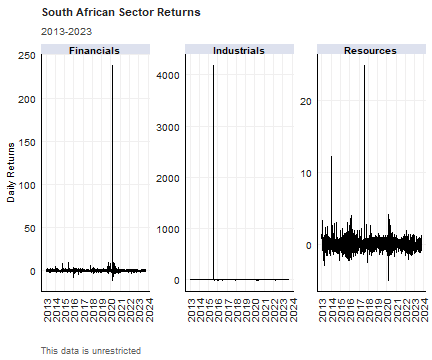
\includegraphics{Essay_files/figure-latex/Figure2-1} 

}

\caption{Cumulative Sector Returns (unrestricted data set) \label{Figure2}}\label{fig:Figure2}
\end{figure}

Table 4.1 provides the descriptive statistics for each of the sector
returns -- this is done on the unrestricted data. The high kurtosis
levels indicate that the returns are leptokurtic. However, looking at
the descriptive data in Table 4.2, the results are more representative
of the price movements.

\% latex table generated in R 4.2.2 by xtable 1.8-4 package \% Wed Jan
31 16:25:20 2024

\begin{table}[ht]
\centering
\begin{tabular}{rlrrr}
  \hline
 & Statistics & Financials & Industrials & Resources \\ 
  \hline
1 & Observations & 2684.00 & 2684.00 & 2684.00 \\ 
  2 & NAs & 0.00 & 0.00 & 0.00 \\ 
  3 & Minimum & -11.04 & -8.61 & -4.93 \\ 
  4 & Quartile 1 & -0.33 & -0.49 & -0.33 \\ 
  5 & Median & 0.12 & 0.13 & 0.05 \\ 
  6 & Arithmetic Mean & 0.32 & 3.25 & 0.10 \\ 
  7 & Geometric Mean &  &  &  \\ 
  8 & Quartile 3 & 0.59 & 0.76 & 0.47 \\ 
  9 & Maximum & 238.16 & 4186.93 & 24.97 \\ 
  10 & SE Mean & 0.13 & 2.21 & 0.02 \\ 
  11 & LCL Mean (0.95) & 0.08 & -1.07 & 0.06 \\ 
  12 & UCL Mean (0.95) & 0.57 & 7.58 & 0.14 \\ 
  13 & Variance & 43.44 & 13058.35 & 1.11 \\ 
  14 & Stdev & 6.59 & 114.27 & 1.05 \\ 
  15 & Skewness & 34.98 & 36.59 & 10.87 \\ 
  16 & Kurtosis & 1258.74 & 1336.70 & 239.48 \\ 
   \hline
\end{tabular}
\caption{Descriptive Statistics Table} 
\label{tab1: DS}
\end{table}

\% latex table generated in R 4.2.2 by xtable 1.8-4 package \% Wed Jan
31 16:25:20 2024

\begin{table}[ht]
\centering
\begin{tabular}{rlrrr}
  \hline
 & Statistics & Financials & Industrials & Resources \\ 
  \hline
1 & Observations & 2684.00 & 2684.00 & 2684.00 \\ 
  2 & NAs & 0.00 & 0.00 & 0.00 \\ 
  3 & Minimum & -11.04 & -8.61 & -4.93 \\ 
  4 & Quartile 1 & -0.33 & -0.49 & -0.33 \\ 
  5 & Median & 0.12 & 0.13 & 0.05 \\ 
  6 & Arithmetic Mean & 0.16 & 0.14 & 0.09 \\ 
  7 & Geometric Mean &  &  &  \\ 
  8 & Quartile 3 & 0.59 & 0.76 & 0.47 \\ 
  9 & Maximum & 13.00 & 13.00 & 13.00 \\ 
  10 & SE Mean & 0.02 & 0.02 & 0.02 \\ 
  11 & LCL Mean (0.95) & 0.11 & 0.10 & 0.06 \\ 
  12 & UCL Mean (0.95) & 0.20 & 0.19 & 0.12 \\ 
  13 & Variance & 1.41 & 1.58 & 0.78 \\ 
  14 & Stdev & 1.19 & 1.26 & 0.88 \\ 
  15 & Skewness & 1.56 & 0.80 & 4.37 \\ 
  16 & Kurtosis & 27.58 & 14.87 & 60.77 \\ 
   \hline
\end{tabular}
\caption{Descriptive Statistics Table (restricted)} 
\label{tab1: DS}
\end{table}

The MarchTest is used to test if there is a need for the MV-GARCH model.
The p-values of all the Marchtests indicate that the GARCH model is
appropriate to use for the data. There is significant autocorrelation
present, which further supports the need for a GARCH model. The MV-GARCH
model is most appropriate for identifying how each sector responds to
shocks and if other sectors are exposed to this shock. This model will
provide valuable information to investors who want to identify the risk
of holding stocks that display co-movement during common and/or unique
sector shocks, as this information helps with hedging purposes and
portfolio diversification. The BEKK (Baba, Engle, Kraft and Kroner)
(Hassan \& Malik (\protect\hyperlink{ref-HassanSyedAun2007MGmo}{2007}))
test is a type of GARCH model that is used for estimating the
conditional variance between each sector. Furthermore, the BEKK model is
limited to handling a maximum of three variables at a time, as this
means that 24 parameters need to be estimated. This model is a type of
GARCH model that Hassan and Malik (2007) use in their paper to identify
volatility transmission (Hassan \& Malik
(\protect\hyperlink{ref-HassanSyedAun2007MGmo}{2007})).

\hypertarget{empirical-results}{%
\section{Empirical Results}\label{empirical-results}}

Three sectors in South Africa are investigated using the MV-GARCH model
with BEKK parameters. These results are presented in Table 5.1 and Table
5.2, with each representing the unrestricted and restricted data sets.
The BEKK parametrisation identifies the conditional variance of each
sector and the conditional covariance between each sector and can
provide some insight into the effect of news through the error/residual
term.

\% latex table generated in R 4.2.2 by xtable 1.8-4 package \% Wed Jan
31 16:25:20 2024

\begin{table}[ht]
\centering
\begin{tabular}{rlrrrl}
  \hline
 & Coefficient & Estimate & Std.Error & t.value & Pr \\ 
  \hline
1 & mu1.Financials & 0.32 & 0.33 & 0.98 & 0.32536315 \\ 
  2 & mu2.Industrials & 3.25 & 3.02 & 1.08 & 0.28063270 \\ 
  3 & mu3.Resources & 0.10 & 0.26 & 0.38 & 0.70138429 \\ 
  4 & A011 & 6.59 &  &  & NaN \\ 
  5 & A021 & -0.05 & 2.22 & -0.02 & 0.98156858 \\ 
  6 & A031 & 0.07 & 0.12 & 0.57 & 0.57078451 \\ 
  7 & A022 & 114.27 &  &  & NaN \\ 
  8 & A032 & -0.03 & 0.07 & -0.37 & 0.71046912 \\ 
  9 & A033 & 1.05 & 0.10 & 10.70 & 2.22e-16*** \\ 
  10 & A11 & 0.10 & 0.01 & 9.75 & 2.22e-16*** \\ 
  11 & A21 & 0.02 & 0.08 & 0.24 & 0.81099501 \\ 
  12 & A31 & 0.02 & 0.01 & 2.86 & 0.00422241** \\ 
  13 & A12 & 0.02 & 0.01 & 3.82 & 0.00013261*** \\ 
  14 & A22 & 0.10 & 0.01 & 11.22 & 2.22e-16*** \\ 
  15 & A32 & 0.02 & 0.00 & 5.12 & 3.0281e-07*** \\ 
  16 & A13 & 0.02 & 0.18 & 0.11 & 0.91128638 \\ 
  17 & A23 & 0.02 & 1.62 & 0.01 & 0.99015553 \\ 
  18 & A33 & 0.10 & 0.19 & 0.51 & 0.60787898 \\ 
  19 & B11 & 0.80 & 0.01 & 68.89 & 2.22e-16*** \\ 
  20 & B21 & 0.02 & 0.13 & 0.15 & 0.87879699 \\ 
  21 & B31 & 0.02 & 0.01 & 1.92 & 0.05512446 \\ 
  22 & B12 & 0.02 & 0.00 & 51.53 & 2.22e-16*** \\ 
  23 & B22 & 0.80 & 0.01 & 121.59 & 2.22e-16*** \\ 
  24 & B32 & 0.02 &  &  & NaN \\ 
  25 & B13 & 0.02 & 0.02 & 1.24 & 0.21510030 \\ 
  26 & B23 & 0.02 & 0.15 & 0.13 & 0.89686714 \\ 
  27 & B33 & 0.80 & 0.01 & 83.42 & 2.22e-16*** \\ 
   \hline
\end{tabular}
\caption{BEKK11 Model} 
\label{tab:bekk11}
\end{table}

\% latex table generated in R 4.2.2 by xtable 1.8-4 package \% Wed Jan
31 16:25:20 2024

\begin{table}[ht]
\centering
\begin{tabular}{rlrrrl}
  \hline
 & Coefficient & Estimate & Std.Error & t.value & Pr \\ 
  \hline
1 & mu1.Financials & 0.17 & 0.02 & 10.67 & 2.22e-16*** \\ 
  2 & mu2.Industrials & 0.22 & 0.02 & 11.65 & 2.22e-16*** \\ 
  3 & mu3.Resources & 0.05 & 0.02 & 3.11 & 0.00188300** \\ 
  4 & A011 & 0.24 & 0.03 & 8.01 & 1.1102e-15*** \\ 
  5 & A021 & 0.35 & 0.10 & 3.56 & 0.00037423*** \\ 
  6 & A031 & 0.28 & 0.07 & 4.09 & 4.3256e-05*** \\ 
  7 & A022 & 0.29 & 0.10 & 2.97 & 0.00294364** \\ 
  8 & A032 & 0.17 & 0.12 & 1.42 & 0.15656910 \\ 
  9 & A033 & 0.60 & 0.02 & 23.85 & 2.22e-16*** \\ 
  10 & A11 & 0.55 & 0.03 & 16.27 & 2.22e-16*** \\ 
  11 & A21 & 0.01 & 0.02 & 0.83 & 0.40656331 \\ 
  12 & A31 & 0.06 & 0.01 & 4.41 & 1.0297e-05*** \\ 
  13 & A12 & 0.05 & 0.02 & 3.06 & 0.00221959** \\ 
  14 & A22 & 0.61 & 0.03 & 22.75 & 2.22e-16*** \\ 
  15 & A32 & 0.01 & 0.01 & 0.97 & 0.33015808 \\ 
  16 & A13 & 0.01 & 0.02 & 0.71 & 0.47599918 \\ 
  17 & A23 & 0.05 & 0.02 & 2.52 & 0.01185218* \\ 
  18 & A33 & 0.52 & 0.03 & 18.93 & 2.22e-16*** \\ 
  19 & B11 & 0.52 & 0.02 & 22.52 & 2.22e-16*** \\ 
  20 & B21 & -0.50 & 0.03 & -15.80 & 2.22e-16*** \\ 
  21 & B31 & 0.09 & 0.04 & 2.38 & 0.01712790* \\ 
  22 & B12 & 0.41 & 0.02 & 20.30 & 2.22e-16*** \\ 
  23 & B22 & 0.85 & 0.03 & 24.52 & 2.22e-16*** \\ 
  24 & B32 & -0.03 &  &  & NaN \\ 
  25 & B13 & -0.26 & 0.03 & -9.00 & 2.22e-16*** \\ 
  26 & B23 & -0.09 & 0.10 & -0.93 & 0.35273150 \\ 
  27 & B33 & 0.00 &  &  & NaN \\ 
   \hline
\end{tabular}
\caption{BEKK11 Model (restricted data)} 
\label{tab:bekk11}
\end{table}

\begin{quote}
The table can be interpreted as follows:\\
Significance codes: 0 = *** \& 0.001 = ** \& 0.05 = *\\
Financials = 1\\
Industrials = 2\\
Resources = 3\\
\emph{eg: A21 refers to the spillover effects of the Industrial sector
on the Financial Sector}
\end{quote}

\newpage

The mean equations represent the expected return from each sector, with
the null hypothesis representing a mean return of zero -- these
estimates are \emph{mu.financials, mu.industrials, mu.resources} in both
tables. Table 5.1 provides statistically insignificant mean returns for
each sector, which means that there is not enough evidence to reject the
null hypothesis. The restricted data set mean returns, as seen in Table
5.2, are statistically significant for all sectors (p-value \textless{}
0.05).

Understanding volatility persistence within each sector provides the
investor with an understanding of how long to expect periods of
irregular movement. The volatility persistence is estimated using the
lagged squared standardised residuals -- these estimates are from
\emph{A011} to \emph{A033} in both tables. This analyses how much of the
current volatility is conditional on past movements. The \emph{A011},
\emph{A022} and \emph{A033} estimates (Table 5.1) indicate the
volatility persistence for each sector, with the industrial sector
displaying the highest levels of persistence. These same estimates from
the restricted data set (Table 5.2) are all statistically significant
(p-value \textless{} 0.05) and positive. Volatility persistence from the
industrial and resource sectors remains persistent in the financial
sector, as \emph{A021} and \emph{A031} are statistically significant
(p-value \textless{} 0.05). These coefficients provide the investor with
an idea of how long volatility will remain in each sector and how much
from other sectors will persist.

\emph{A11} is a matrix coefficient that represents the volatility
spillovers between sectors -- these estimates are from \emph{A11} to
\emph{A33} in both tables. It indicates the extent to which the past
historical data influences the current covariance between and within
each sector. The restricted data (Table 5.1) indicates that only five of
the variables are significant (p-value \textless{} 0.05), with all
estimates being positive. The financial sector is affected by volatility
spillover from the resource sector ( \emph{A13} p-value). The industrial
sector is vulnerable to volatility spillover from the financial and
resource sectors, with each having an equal impact (equal estimates from
\emph{A21} \& \emph{A23}) and the resource sector being more
statistically significant. The resource sector is unperturbed by any
volatility from the other sectors (p-value \textgreater{} 0.05). The
restricted data results (Table 5.2) have six significant variables
present and all estimates are positive. The financial sector is
vulnerable to volatility spillover from the resource sector, as the
p-value is significant ( \emph{A31}). Volatility in the financial sector
is transmitted to the industrial sector, indicated by the significant
p-value ( \emph{A12}), but the converse is not present. Lastly, the
resource sector remains unaffected by volatility movement in the other
sectors. The volatility spill-over indicator provides invaluable
information to an investor, as holding any financial or industrial
sector equity requires constant vigilance of the other sectors, whereas
the resource sector is unaffected. This information remains constant for
both data sets.

The B matrix coefficients provide the shock impact of each sector. This
is interpreted as the ability of the sector to deal with news from its
own and other sectors -- these estimates are from \emph{B11} to
\emph{B33} in both tables. Table 5.1\} only contains positive estimates,
for the B coefficients, but only four of these estimates are significant
at the five per cent level. The financial sector is significantly
affected by news from its sector. Furthermore, although the p-value from
the resource sector is not significant (p-value = 0.055), it can be
substantiated that the resource sector news impacts the financial
sector. The industrial sector is influenced by shocks from its sector
and the financial sector (p-value \textless{} 0.05). Lastly, the shock
impact on the resource sector is only affected by news from its sector.
Table 5.2 comprises a mix of positive and negative estimates of which
six of them are significant at the five percent level. The financial
sector is highly influenced by news in its sector and from the other two
sectors, as all p-values are significant at the five per cent level. The
industrial and resource sector news each respectfully has a positive and
negative impact on the financial sector, with the former having a
greater effect. The industrial sector is positively impacted by its
shocks and shocks from the financial sector, with an unfortunate
\emph{NaN} for the resource impact. The resource sector's news impact
cannot be interpreted, as a \emph{NaN} is present, but any shock to the
financial sector is significant and negatively impacts this sector.
These findings are important to investors, as they can better understand
the impact that shocks (endogenous and exogenous) have on sectors.

\hypertarget{conclusion}{%
\section{Conclusion}\label{conclusion}}

Since the introduction of the GARCH model, there have been several
iterations of it, each slightly different, to provide the user with more
sensible and robust estimates. The world of finance research and
understanding of variance has been greatly improved using
heteroskedastic conditional variance modelling. Logically, during
economic swings or exogenous and/or endogenous shocks, it makes sense to
expect local equity prices to remain in a volatile state
(i.e.~volatility clustering), this is taken into consideration for the
risk/variance estimates. Volatility modelling has been sought after by
many researchers, as identifying the closest estimate of deviation
compared to the actual change in listed price allows for better
portfolio optimisation. The BEKK parametrisation is a version of the
MV-GARCH model that breaks down the volatility between three variables
of interest and provides a much deeper understanding of volatility
persistence, spillover and reaction to shocks.

This paper's findings indicate that although the South African economy
is faced with a multitude of economic issues, the volatility created by
this is identified with the use of the MV-GARCH model. The empirical
findings are of great use to investors who want to hold local equities
from the financial, industrial and resource sectors. The results can
illustrate the source of volatility in their sector and how long it will
remain (persistence), whether the volatility is carried over to another
sector (spillover), and how well each sector can deal with shocks. These
findings are invaluable for portfolio optimisation and deliver a better
understanding of the resilience of these sectors in the South African
climate.

This research can be expanded upon by including more key economic
sectors of South Africa, as this will further help investors with
portfolio optimisation, hedging and many more applications. However,
this paper can be improved by dealing with the NaNs present in the data,
as it will help identify which independent variable estimates are
statistically significant (p-value \textless{} 0.05).

\newpage

\hypertarget{references}{%
\section*{References}\label{references}}
\addcontentsline{toc}{section}{References}

\hypertarget{ref.bib}{}

\hypertarget{refs}{}
\begin{CSLReferences}{1}{0}
\leavevmode\vadjust pre{\hypertarget{ref-RePEc:pra:mprapa:80763}{}}%
Bakari, S. 2017. \emph{{Why is South Africa Still a Developing
Country?}} (MPRA Paper 80763). University Library of Munich, Germany.
{[}Online{]}, Available:
\url{https://ideas.repec.org/p/pra/mprapa/80763.html}.

\leavevmode\vadjust pre{\hypertarget{ref-world2020global}{}}%
Bank, W. 2020. \emph{Global investment competitiveness report 2019/2020:
Rebuilding investor confidence in times of uncertainty}. The World Bank.

\leavevmode\vadjust pre{\hypertarget{ref-BollerslevTim2023RoGA}{}}%
Bollerslev, T. 2023. Reprint of: Generalized autoregressive conditional
heteroskedasticity. \emph{Journal of econometrics}. 234:25--37.

\leavevmode\vadjust pre{\hypertarget{ref-BurnsPatrick1998CaVo}{}}%
Burns, P., Engle, R.F. \& Mezrich, J.J. 1998. Correlations and
volatilities of asynchronous data. \emph{The Journal of derivatives}.
5(4):7--18.

\leavevmode\vadjust pre{\hypertarget{ref-EngleRobert2001G1TU}{}}%
Engle, R. 2001. GARCH 101: The use of ARCH/GARCH models in applied
econometrics. \emph{The Journal of economic perspectives}.
15(4):157--168.

\leavevmode\vadjust pre{\hypertarget{ref-EngleRobertF.1982ACHw}{}}%
Engle, R.F. 1982. Autoregressive conditional heteroscedasticity with
estimates of the variance of united kingdom inflation.
\emph{Econometrica}. 50(4):987--1007.

\leavevmode\vadjust pre{\hypertarget{ref-HassanSyedAun2007MGmo}{}}%
Hassan, S.A. \& Malik, F. 2007. Multivariate GARCH modeling of sector
volatility transmission. \emph{The Quarterly review of economics and
finance}. 47(3):470--480.

\end{CSLReferences}

\bibliography{Tex/ref}





\end{document}
